\documentclass{article}
\usepackage{biblatex}
\usepackage[utf8]{inputenc}
\usepackage[a4paper]{geometry}
\usepackage{hyperref}
\usepackage{caption}
\usepackage{graphicx}
\usepackage{float}
\usepackage{todonotes}
\usepackage{amsmath}
\usepackage{subcaption}
\title{Truth teller's dice}
\author{Ruurd Bijlsma (S3860469) \\
Bharath Kumar Musuadhi Rajan (S4065476) \\
Jordi Timmermans (s3870758)
}

\begin{document}

\maketitle

\section*{Introduction}

We have implemented a modified version of the game "Liar’s dice" using epistemic logic. We have retained the core concept and playing rules of the original game but modified the bidding condition of the agents. Unlike the original game, where players can bid for scenarios knowing that it would not be possible, the agents in our version of the game can only place bids that they consider possible with respect to their knowledge. We have also simplified it by limiting the number of sides per die, and the number of dice per player. The goal of the project is to explore and analyse different strategies that would emerge as a result of modelling the game using epistemic logic. We outline a few strategies later in this report. We run the game multiple times with varying strategies for each agent, to test which strategy works best. We display the player's knowledge in the form of agents' knowledge in epistemic logic syntax, along with the Kripke model. A game simulation to better understand the game and explain why some strategy works better.

\begin{figure}[h]
    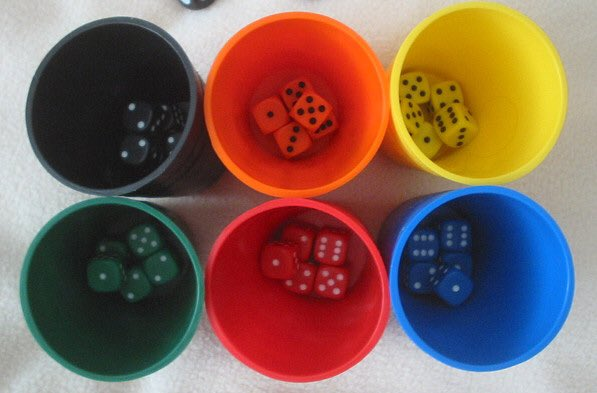
\includegraphics[width=0.9\textwidth]{img/Er3haXVXEAYrp0r.jpg}
    \centering
    \caption{Liar's Dice}
    \label{fig:liarsdice}
\end{figure}

\section*{Game description}
Liar's dice is a dice game for two or more players. Each player starts with a set number of dice. All players roll once, after which the players take turns bidding a number of dice and the number of pips of those dice. Each player can either make a bid or challenge the previous bid. A bid is challenged when the player does not consider the previous bid possible or guesses the number of dice for that number of pips is too high. When a challenge is made, the player calls out that the previously made bid is false and everyone must reveal their dice. If the challenge is correct (i.e., the number of dice for the number of pips that make up the bid exceeds what the players combined have), then the player who made the bid, loses one of their dice and the next round starts. If the challenge is incorrect however, the challenging player loses a die.

During Liar's dice a big part of the game is bluffing your bid, to not reveal information about your hand. In Truth teller's dice, there is no lying, meaning every bid must be something the agent considers possible.

\subsection*{Elements of the game} %ruurd
\begin{enumerate}
    \item 2 or more players
    \item N number of dice for each player
    \item 2 or more sides per die
\end{enumerate}
\subsection*{Setup} %ruurd
At the start of each round every player rolls their dice and only looks at them their selves, no one else can see it.

\subsection*{Gameplay Rules} %ruurd
An agent can make a bid based on what it knows to be possible. A bid consists of a face value of the die, along with the total number of dice on the deck with that face value. For example, an agent can bid that there are two dice with the face value “1” on them. There are two types of bids that an agent can be make, 1) A bid that increases the quantity of dice retaining the number of pips (face value) of the previous bid, or 2) A bid that increases the number of pips retaining the current dice quantity. If one increases the pips, that player is able to call the number of dice starting from 1 again.

After each bid, the next agent decides whether it should challenge the previous bid, or to continue with a new bid. If the agent thinks that the previous bid is impossible, then it challenges the bid, else the agent makes a new bid that it considers to be possible. 

When the agent decides to make a challenge, the round ends and all the agents reveals their dice. If the challenge is correct, the challenged player will lose a die, and a new round starts. If the challenge is not correct, meaning the previous bid was actually correct, then the challenger loses a die and the round restarts.

\subsection*{End of game} %ruurd
The game ends when only one agent is left with some dice, this agent is the winner of the game.

\section*{Game implementation}
\subsection*{Initial configuration}
First, an initial world list is created where all possible combinations of dice get listed. From these initial worlds, a connection matrix is set up where every element is the connection between two worlds. These elements contain which agent is not able to distinguish the two worlds. Besides this, two empty knowledge bases are initiated: one containing the logical knowledge of the agents and the other containing the bids.

In the next step, the agents’ dice are rolled, and each agent knows the outcomes of its own dice roll. The connection matrix gets updated based on the knowledge of the agent. The output of the server during the initial game state can be seen in figure \ref{fig:initc}. The connection matrix stores what links there are in the Kripke model, in the figure shown below the value of every cell is 123, this means that every world is connected to every other world by all agents. The 123 refers to agents 1, 2, and 3, and the rows and columns refer to the worlds.
\begin{figure}[h!]
    \centering
    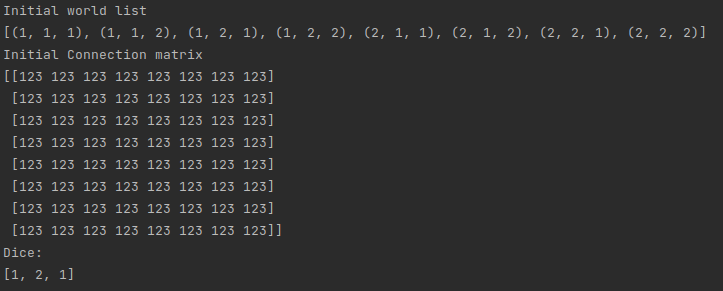
\includegraphics[width=\textwidth]{img/initialconfig.png}
    \caption{Initial configuration using 3 players, 1 die per player and 2 sides per die}
    \label{fig:initc}
\end{figure}
\subsection*{Rounds}
The first agent initiates the game by making a bid based on the rules mentioned in the Gameplay rules section. The knowledge base of the bids and the logic gets updated as the game progresses, with each agent making a new bid.  Since the bids are made based on the possible world scenarios with respect to that agent, when an agent, say Agent-1 bids the maximum amount of a specific pip, the other two agents know what dice player-1 has (namely all dice of that player are dice of the bid number of pips). Therefore, the connection matrix gets updated accordingly. When the next agent, say Agent-2, does not challenge the bid, the other two agents also know what dice Agent-2 has, so the matrix gets updated again.

If an agent loses a challenge or loses to a challenge, that agent loses a die, and everything gets reinitiated.


An example of how a part of a round plays out can be seen in figure \ref{fig:halfaround}. The "quantities" refer to the highest bid per pip until now. So $[1\ 2]$ means the players maximally bid 1 on 1 pip and 2 on 2 pips.
\begin{figure}[h!]
    \centering
    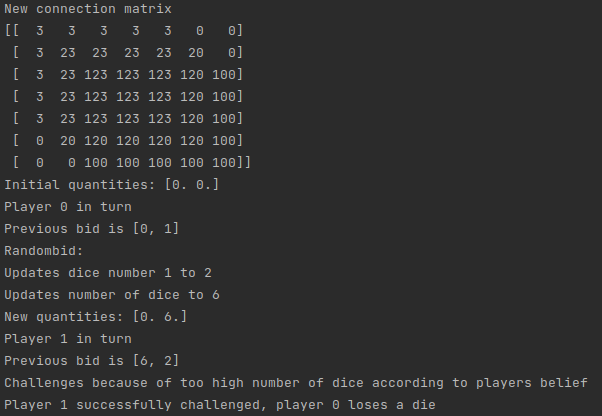
\includegraphics[width=.6\textwidth]{img/gameplay.png}
    \caption{Server showing the output after players looked at their dice and after player 0 announced a bit to update the number of dice with 2 pis to 6. The elements of the connection matrix show which player can't differentiate between worlds on the horizontal axis and the vertical axis (not shown in the screenshot).}
    \label{fig:halfaround}
\end{figure}

\subsection*{Client-server connection} %ruurd
We implemented this project in two parts, the client as a web application, and the server as a Python program. This is because a user interface is easier to create in the web, and the logic part is easier to create in Python. The two parts communicate through WebSockets, the client connects to the server and sends a 'start game' event, the server then starts a game and saves it for this client, the server then sends information about the game through events to the client. The client can still request extra information or give commands through events, because an instance of the game is saved per client. 

\subsection*{Client}
The client shows the Kripke model, the game state, the logical atoms per step, actions to interact with the server, and a round and step selector so the user can choose which state to view. The round selector in the top right of \autoref{fig:screenshot} shows five rounds. The user can click these buttons to view that round. The panels below then update their contents to show information for that given round. The different steps made in this round are shown in the bottom panel. The right panel shows the Kripke model, in this panel the user can choose which step to visualize. The meaning of each step is given in the bottom panel named "Round steps". In \autoref{fig:screenshot} the fourth step is selected, meaning the Kripke model shown also reflects the fourth step from the "Round steps" panel, namely it shows the state after Player 2 has bid (5 * 1).

The client also contains some buttons and selectors to interact with the server. The selectors let the user configure what strategy to use, how many dice to use, how many players there are, and how many dice sides to use. With this configuration, the user can choose to start a new game or to simulate a given number of games. The user can also simulate games in the client with the simulate tab. There the user chooses a game configuration (number of player, sides, dice, and strategy) and choose how many games to simulate. The amount of times each player has won a game is then shown.

\begin{figure}[h]
    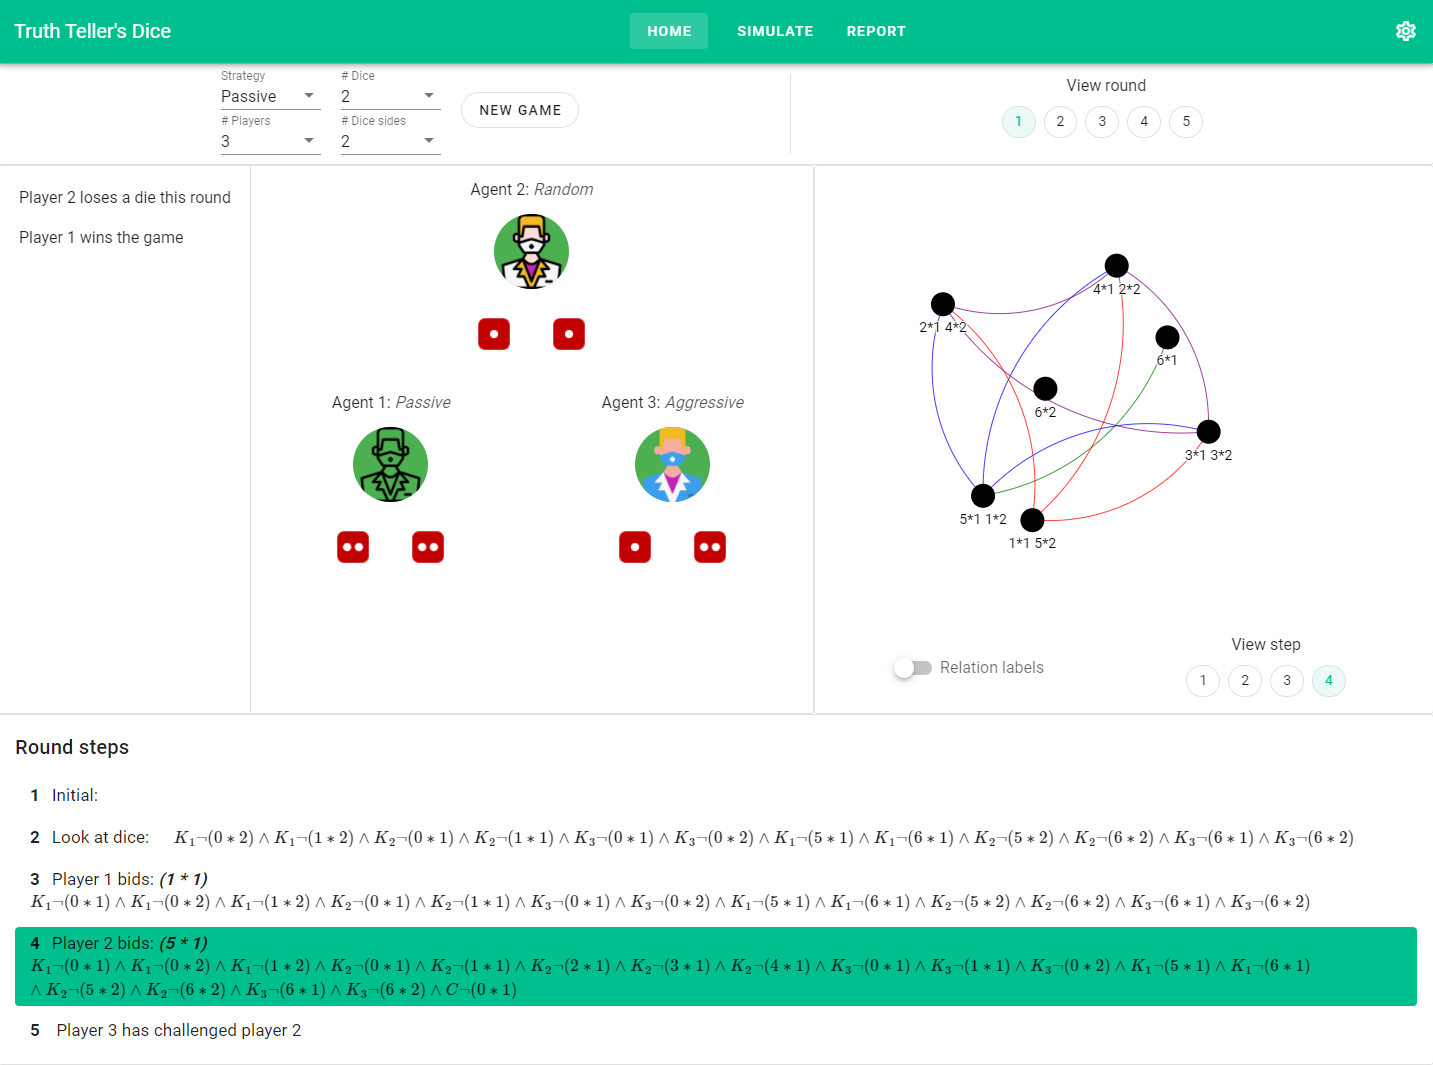
\includegraphics[width=\textwidth]{img/imgscreenshot.png}
    \centering
    \caption{Client user interface visualizing the model, game state, and logical atoms after one bid have been made.}
    \label{fig:screenshot}
\end{figure}

\subsection*{Model visualization} %Ruurd
The model is visualized in the client using d3.js. The labels for the relations can be toggled, and it is possible to switch between Kripke models representing steps. This example model shows a game with two-sided dice, two dice per player, and three players. The labels for the worlds show what dice are rolled for all players combined in that world. The unconnected worlds are worlds that are not possible anymore, no player considers them possible. For example, we can see in the round steps at the bottom of \autoref{fig:screenshot} that $K_1 \neg (6*1) \land K_2 \neg (6*1) \land K_3 \neg (6*1)$. This is reflected in the model, (6*1) is an unconnected world.

\begin{figure}[h]
    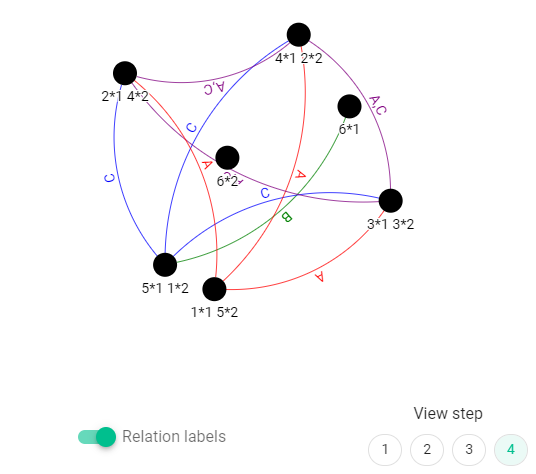
\includegraphics[width=.5\textwidth]{img/withrelations.png}
    \centering
    \caption{Kripke model with labels showing which agent can use the relation.}
    \label{fig:screenshot}
\end{figure}

\subsection*{Round steps}
At the bottom of the client UI the knowledge is printed using epistemic logic syntax. In \autoref{fig:screenshot} we can see this knowledge base after each step. After each player has look at their dice, some knowledge is gained and after any player makes a bid everyone's knowledge is updated. In this case, because the bid was (5*1), it becomes common knowledge that (0*1) is not true $C \neg(0*1)$. The highlighted step of "round steps" is synchronized with the selected step in the Kripke model panel.

\subsection*{Game visualization}% bharat
The gameplay simulation can be visualized alongside the model visualization. The VueJS framework allows to specify the layout of the elements in the game visuals using HTML5, and also allows to update the agents, their strategy and their respective dice for each new game via JavaScript. Once the game is started, the visuals are updated based on the \textit{Rounds} chosen by the user from the 'View Round' option. This dynamic behaviour of the visual elements, i.e., reading the information from the server and updating in the client, is made with the help of the aforementioned socket.io library. 

%\todo{}

% \begin{figure}[h]
%     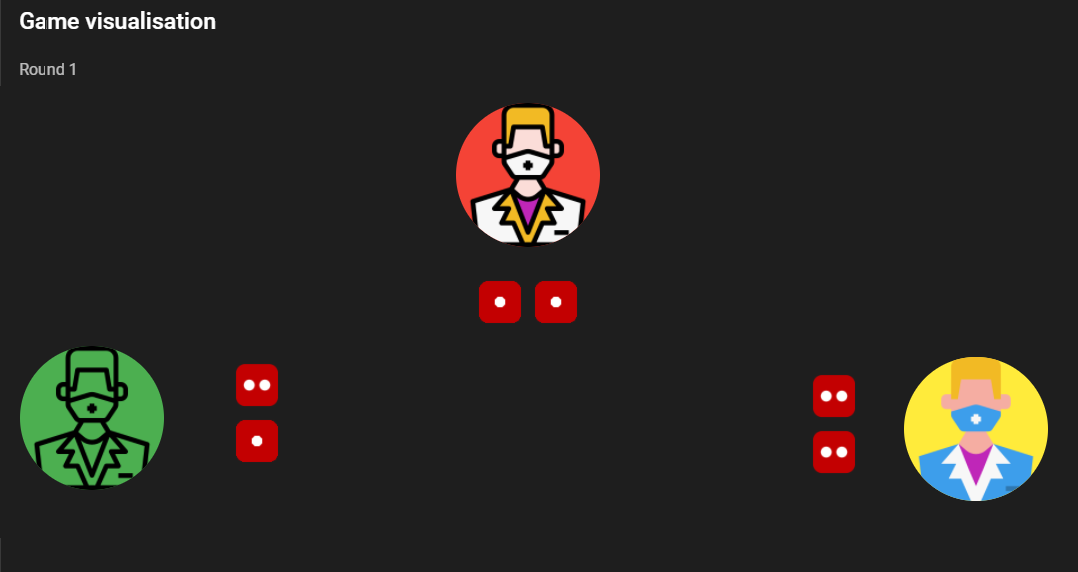
\includegraphics[width=0.8\textwidth]{img/GV1.png}
%     \centering
%     \caption{Game visualization at the initial stage when the dice are rolled}
%     \label{fig:liarsdiceGV}
% \end{figure}



\section*{Logical modelling}
\subsection*{Example of a game}
\begin{enumerate}
    \item A game with 3 players, each with three 3-sided dice, will have a combination of the following atoms, initially adding up to 9:\\
    (0*1), (1*1), (2*1), (3*1), ..., (9*1)\\
    (0*2), (1*2), (2*2), (3*2), ..., (9*2)\\
    (0*3), (1*3), (2*3), (3*3), ..., (9*3)\\
    \item In this situation there are 9 dice in total, and 3 sides per dice. In a Kripke model every world represents what dice there are in total, for example, one world could be $(5*1, 3*2, 1*3)$. The number of worlds is equal to the uniques of all combinations of dice. A simplified example: with four total dice and two sides the possible worlds are
    \begin{itemize}
        \item (4*1)
        \item (3*1), (1*2)
        \item (2*1), (2*2)
        \item (1*1), (3*2)
        \item (4*2)
    \end{itemize}
    \item Before looking at their own dice each agent considers all these atoms possible ($M_a(0*1)$, ..., $M_c(9*3)$)
    \item Each agent gets to know what dice they rolled through a private announcement. After this announcement, each agent can eliminate some possibilities (if agent B has $[1, 1, 2]$ as dice, then $K_b \neg (9 * 3)$, $K_b \neg (8 * 3)$, $K_b \neg (7 * 3)$, $K_b \neg (9 * 1)$, $K_b \neg (9 * 2)$, $K_b \neg (8 * 2)$.). Some relations between worlds in the Kripke model could be cut after the announcement.
    \item The game starts when the first player makes a bid, for example, agent A announces he considers it possible that there are seven dice with a three on on it. This makes it common knowledge that agent A considers this is possible, so $CM_a(7 * 3)$.
    \item Because now every agent knows that agent a considers (7 * 3) possible, every agent now also knows agent A has at least one die with a three (because there are only 9 dice in total, and agent A has three of them. $C \neg (0 * 3)$, it's now common knowledge that (0 * 3) is impossible. Agents that have a 3 themselves are able to eliminate more possibilities. 
    \item After agent A's bid, it's now agent B's turn. Agent B knows (7 * 3) is not possible ($K_b \neg (7 * 3)$ from (3)), so agent B must challenge the previous bid.
    \item After agent B's challenge, everyone reveals their dice and agent A will lose one die because he made a bid that turned out not to be true. This goes on until there is only one person with dice left.
\end{enumerate}
\subsection*{Model solver}%Explanation of the model solver here.
The model is solved by keeping track of a matrix that contains the connections for each word. Each element of the matrix initially contains connections for each player. Whenever a player gets more knowledge, the element might be adjusted because a player might be able to differentiate between two worlds. The real world will always contain all the reflexive connections because no one can differentiate between the real world and itself. 
\subsection*{Strategies} %ruurd
We will test multiple strategies for the agents. The strategies are used to decide which bid will be picked out of the possible legal bids, and when to make a challenge.
\subsubsection*{Challenging strategy}
The players in this game are mathematical geniuses and can calculate combinations and summations of those without any issue. The strategy to challenge another player will be based on the number of dice in play and the dice the player holds. The probability of challenging is calculated by $ \sum^{x}_{i=k} \begin{pmatrix}
x\\
k
\end{pmatrix} *(\frac{1}{sides})^i*(1-\frac{1}{sides})^{x-i}$. This calculation is the probability of the bid being satisfied according to the players knowledge. x is the number of dice the others have, k is how many dice are needed to be rolled on the corresponding pip to satisfy the bid. If the probability is for example 30 \%, the player will challenge 70\% of the time.
\subsubsection*{Bidding strategies}
There are three bidding strategies in the game adopted by the players. 
\begin{enumerate}
    \item Passive bid (lowest risk). Increase the pips or amount of dice by the smallest amount possible.
    \item Aggressive bid (highest risk). Always increases the number of pips, and randomly selects a number of dice.
    \item Random bid (random risk). Regardless of the previous bid, randomly pick a legal move.
    % \item Bid one higher than the previous bid. Pick a legal move that is as close as possible to the previous bid.\\
    % If not possible to bid higher, bid one pip higher to 1.
    % \item Random bid. Regardless of the previous bid, randomly pick a legal move.
    % \item Bid as high as possible. Regardless of the previous bid, the agent always bids the highest possible legal move.
    % \item Eliminate as few worlds as possible. Bid whichever legal move would eliminate the fewest possible worlds.
    % \item Eliminate as many worlds as possible. Bid whichever legal move would eliminate the most possible worlds.
\end{enumerate}
% \subsubsection{Challenging strategies}
% -challenges if its too much for players belief\\
% -challenges if player doesnt belief according to probability
% https://math.stackexchange.com/questions/2143399/probability-of-rolling-at-least-n-6s-from-x-dice
\section*{Results}
Players are put up against each other in one vs one's as well as a 4 player game. In the one vs one, all players got 3 dice with 3 sides each and got assigned a random strategy every match. The game is simulated for 10.000 matches. The ratio of successful challenges where player 1 challenges player 2 can be seen in figure \ref{fig:1v1_1c2}, whereas the ratio of successful challenge where player 2 challenges player 1 can be seen in figure \ref{fig:1v1_2c1}
\begin{figure}
     \centering
     \begin{subfigure}[b]{0.49\textwidth}
        \centering
        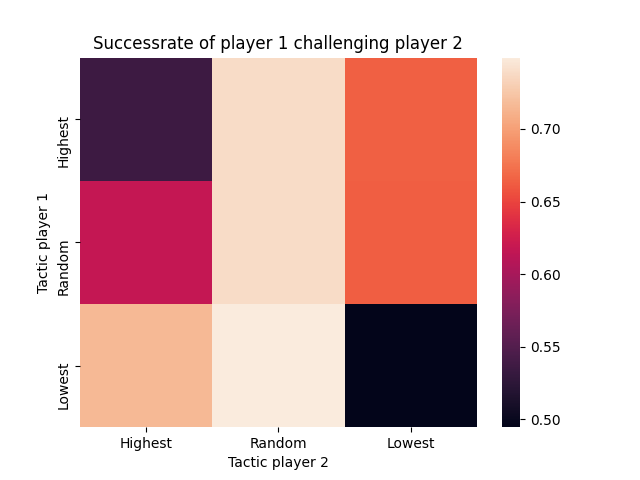
\includegraphics[width=\textwidth]{img/1c2.png}
        \caption{}
        \label{fig:1v1_1c2}
     \end{subfigure}
     \hfill
     \begin{subfigure}[b]{0.49\textwidth}
    \centering
        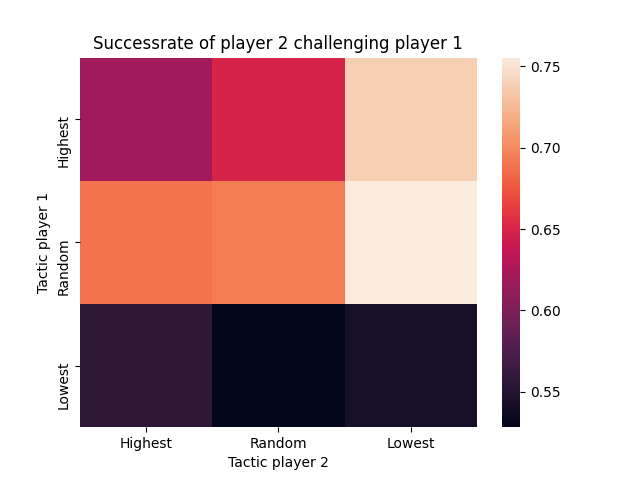
\includegraphics[width=\textwidth]{img/2c1.png}
        \caption{}
        \label{fig:1v1_2c1}
     \end{subfigure}
     \caption{Successful challenge ratio of one player versus another}
     \label{fig:1v1}
\end{figure}\\
We can see that in both cases challenging is advisable against all players. Challenging a passive player when in the 2nd position however is not very profitable. Challenging a player that plays randomly is in both cases very profitable, that is, assuming one is able to calculate the right probabilities. 
The next simulation performed is that of 1000 games with 4 players, 3 dice per player, and 3 sides per dice. The ratio of successful challenges can be seen in figure \ref{fig:success4player}. Here the vertical axis is the challenger and the horizontal axis is the challenged player. 
\begin{figure}
    \centering
    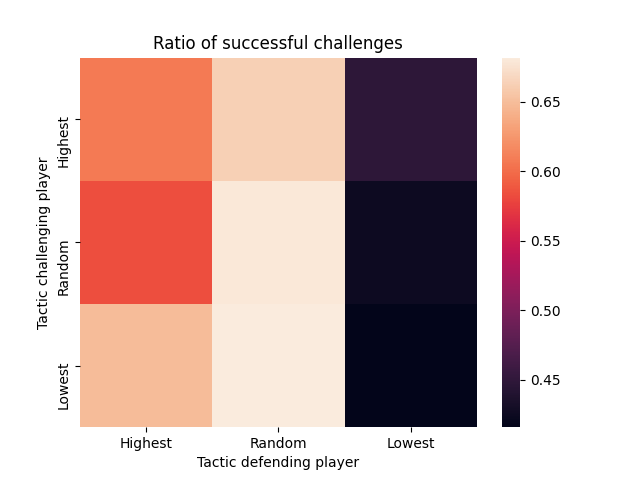
\includegraphics[width=0.8\textwidth]{img/ratio4players.png}
    \caption{Success ratio for challenging in a 4 player game}
    \label{fig:success4player}
\end{figure}\\
Here we can see that challenging a player who takes the lowest risk is not profitable, while challenging a player who randomly takes numbers is very profitable. One reason for this is that the players who play randomly or aggressive tend to update their number of dice to a high number, causing the next player to easily challenge.\\
Besides which tactic is best to use or to challenge, we also took a look at the position in which one challenged to see whether there is a positional advantage. The results can be seen in table \ref{tab:battleroyale}.  

\begin{table}[h!]
    \centering
    \begin{tabular}{c|c|c|c|c}
        &Player1 & Player2 & Player3 & Player4  \\
        \hline
        Challenges per position & 1303 & 5141 & 2185 & 607\\
        Successful challenges per position & 885 & 1684 & 1206 & 449\\
        Successful challenge ratio per position & 0.679 & 0.522 & 0.552 & 0.740\\
    \end{tabular}
    \caption{Positional success rate in a game with 4 players.}
    \label{tab:battleroyale}
\end{table}
We can see that the best positions to be in are the two positions in the middle. The reason for this is that the later one is in position, the more likely it is that the player before him has bid something that he does not consider possible because the bid is impossible according to his knowledge. This for example may peak for player 4 as we can see in the table.
\section*{Conclusion and discussion}
In this game it is very rewarding to play passive because if you do not, you might end up bidding too high and you will get successfully challenged. If you do not like to play passive it seems like the best option for you is to upgrade the pips every turn, since this is more profitable that randomly picking some legal move. If there are multiple players, the best position to be in is the first one, since in our simulations we could see that it has a successful challenge ratio of around $68\%$ and only gets successfully challenged $52\%$ of the time.
% best winrate
% todo list

\section*{Further improvements}
We thought about creating a rule for the agents where they would only be allowed to challenge a bid when they know for a fact that the challenge will succeed. This way the gameplay is more logic based and not based on randomness, but it does stray further from the original Liar's Dice game. This rule would still always result in a game that ends, because the pips or the number of dice always increases in subsequent bids.


%\bibliography{references}
\end{document}
